
%place your content here, feel free to create subcontent files

\begin{block}{\blocktitle{Abstract}}
\justifying
We propose minimum regret search (MRS), a novel acquisition function for Bayesian
optimization. MRS bears similarities with information-theoretic approaches
such as entropy search (ES). However, while ES aims in each query at maximizing the
information gain with respect to the global maximum, MRS aims at minimizing the
expected simple regret of its ultimate recommendation for the optimum. While empirically ES and MRS perform similar in most of the
cases, MRS produces fewer outliers with high simple regret than ES. We provide empirical
results both for a synthetic single-task optimization problem as well as for a
simulated multi-task robotic control problem.
\end{block}

\begin{block}{\blocktitle{Background}}
\textbf{Bayesian optimization} \cite{shahriari_taking_2016}:
\begin{itemize}
\item black-box optimization problems $\mathbf{x} = \arg\min_{\mathbf{x} \in \mathcal{X}} f(x)$ of some function $f: \mathcal{X} \to \mathbb{R}$ on some bounded set $\mathcal{X} \subset \mathbb{R}^D$.
\item maintains a \emph{probabilistic model} $p(f)$ for $f(\mathbf{x})$, typically a Gaussian process (GP)
\item decides on a query point $\mathbf{x}_{n+1}$ where $f$ will be evaluated next based on GP posterior of first $n$ observations $\mathcal{D}_n=\{(\mathbf{x}_i, y_i)\}_{i=1}^n$ and an \emph{acquisition function}
\item recommends $\mathbf{\tilde x}_N$ after $N$ queries (optimum of GP or best query point)
\item objective: minimize \emph{simple regret} 
$R_f(\mathbf{\tilde  x}_N) = f(\mathbf{x}^\star) - f(\mathbf{\tilde  x}_N) = \max_{\mathbf{x}} f(\mathbf{x}) - f(\mathbf{\tilde x}_N)$
\end{itemize}

Acquisition functions decide where to query next:
\begin{itemize}
\item Upper-Confidence Bound (UCB): $a_{UCB}(\mathbf{x};
\mathcal{D}_n) = \mu_{n}(\mathbf{x}) + \kappa_n \sigma_{n}(\mathbf{x})$
\item Probability of Improvement (PI): $a_{PI}(\mathbf{x}; \mathcal{D}_n) := \mathbb{P}[f(\mathbf{x}) > \tau]$
\item Expected Improvement (EI): $a_{EI}(\mathbf{x}; \mathcal{D}_n) := \mathbb{E}[(f(x) - \tau)\mathbb{I}(f(x) > \tau)]$
\item Entropy Search (ES) \cite{hennig_entropy_2012}: $a_{ES}(\mathbf{x}, \mathcal{D}_n)
  = H(\mathbf{x}^\star \vert \mathcal{D}_n) - \mathbb{E}_{y \vert \mathbf{x}, \mathcal{D}_n}
	[H(\mathbf{x}^\star \vert \mathcal{D}_n \cup \{(\mathbf{x}, y))]$,
	where $H(\mathbf{x}^\star \vert \mathcal{D}_n)$ denotes the differential entropy
of the posterior distribution $p^\star(x \vert \mathcal{D}_n)$ of the unknown optimizer $\mathbf{x}^\star = \arg\max_{\mathbf{x} \in \mathcal{X}} f(\mathbf{x})$.
\end{itemize}

\end{block}

\begin{block}{\blocktitle{Minimum Regret Search}}

\begin{itemize}
 \item estimate probability $p_{opt}(\theta)$ that the global optimum of unknown function $f$ is at $\theta$ at finitely many points $\{\theta^c\}_{i=1}^{N_\theta}$ and approximate using Monte Carlo integration
 \item predict the change of GP when drawing a sample at the query point
$\theta^q$ and assuming $N_y$ different outcomes $\{y^{(i)}\}$ sampled from the
GP's predictive distribution at $\theta^q$
 \item select query point that minimizes the average loss (maximizes the relative entropy) $\mathcal{L}(p_{opt}[\theta^q]) = - \int p_{opt}[\theta^q](\theta) \log \frac{p_{opt}[\theta^q](\theta)}{U_I(\theta)}, \text{d}\theta$,  where $p_{opt}[\theta^q]$ denotes the probability
 distribution of the global optimum \emph{after} an assumed query at $\theta^q$.
\end{itemize}

Approximation:
\begin{itemize}
 \item 
 \item $n_f=1000$, $n_r=25$, and $n_y=51$
\end{itemize}
\end{block}

\begin{block}{\blocktitle{Illustration}}
\vspace*{1cm}

\begin{figure}
\centering
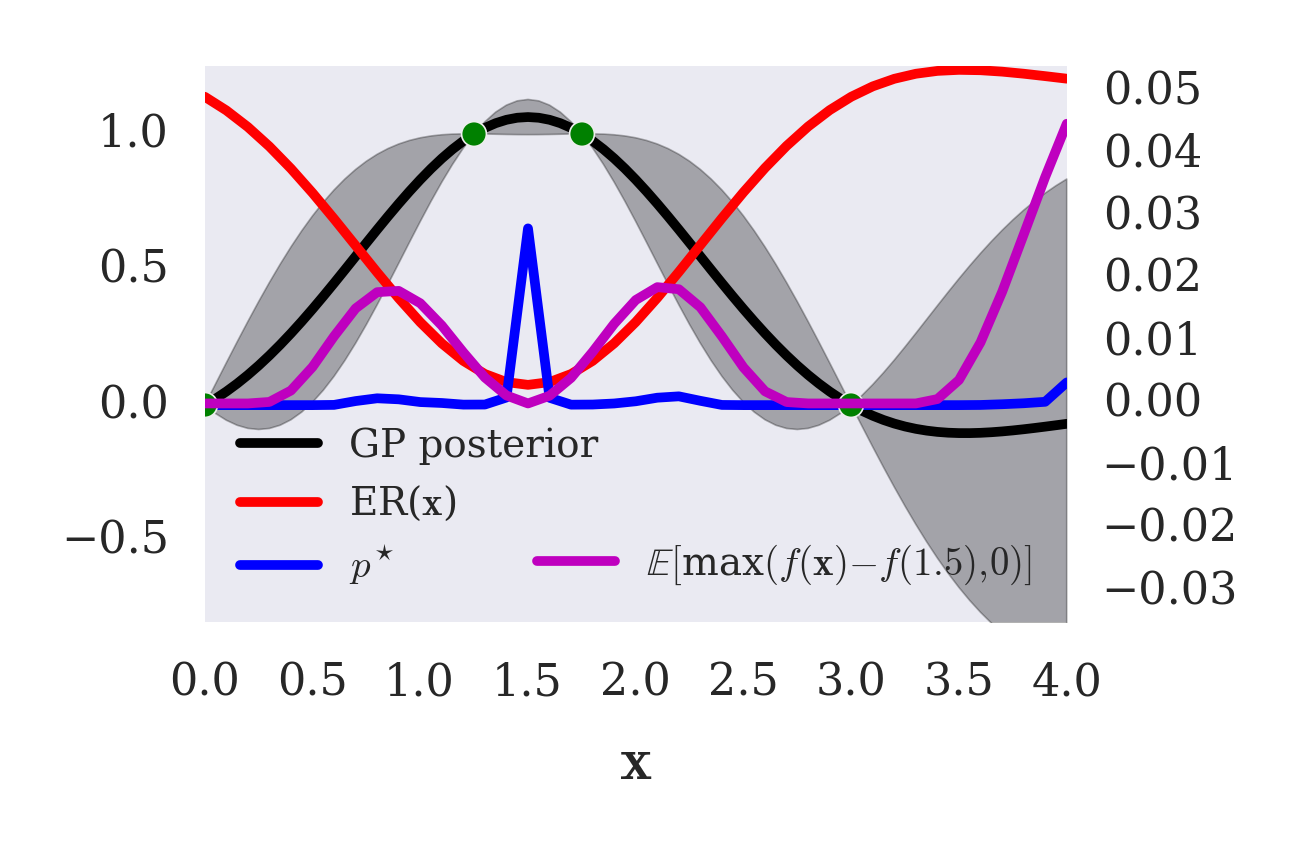
\includegraphics[width=0.48\columnwidth]{../pics/regret_illustration}
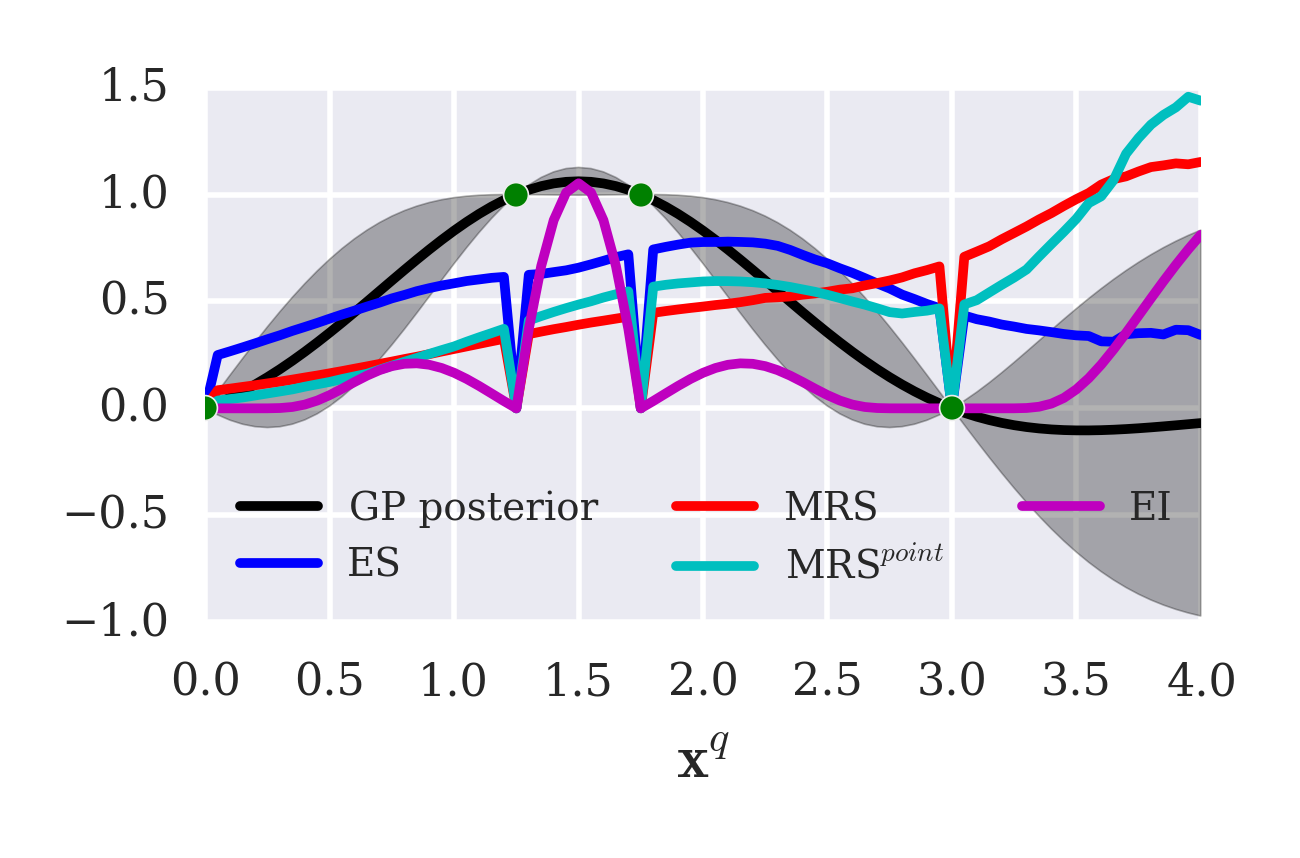
\includegraphics[width=0.48\columnwidth]{../pics/acq_comparison}
\caption{(Left) GP posterior, probability of maximum $p^\star$, expected regret ER, and  $\mathbb{E}[\max(f(\mathbf{x}) - f(1.5), 0)]$ (scale on right-hand side). (Right) GP posterior and different acquisition function. Absolute values have been normalized such that the mean value of acquisition function is $0.5$.}
\label{fig:MRS_illustration}
\end{figure}
\end{block}
